\pdfoutput=1
\pdfminorversion=7

\documentclass[aspectratio=169]{beamer}
% \documentclass{beamer}

\usetheme{metropolis}

% Intel palette
\definecolor{DarkBlue}{HTML}{003C71}
\definecolor{Blue}{HTML}{0071C5}
\definecolor{LightBlue}{HTML}{00AEEF}
\definecolor{Gray}{HTML}{B1BABF}
\definecolor{Orange}{HTML}{FFA300}
\definecolor{Red}{HTML}{FC4C02}
\definecolor{White}{HTML}{FFFFFF}
\setbeamercolor{alerted text}{fg=Blue}
\setbeamercolor{frametitle}{bg=Blue}

\setbeamercolor{palette primary}{fg=White, bg=Blue}

\usepackage{xspace}
\newcommand{\themename}{\textbf{\textsc{metropolis}}\xspace}

\title{The Path to DPDK Speeds for AF\_XDP}
\date{Linux Plumbers Conference, Vancouver, 2018}
\author{magnus.karlsson@intel.com, bjorn.topel@intel.com}
\titlegraphic{\hfill
\includegraphics[width=2cm]{intel-logo.pdf}} 

\begin{document}
  \maketitle

  \begin{frame}{XDP 101}
    \centering\resizebox{!}{.9\textheight}{\input{xdp.pdf_t}}
  \end{frame}
  \begin{frame}{AF\_XDP 101}
    \begin{itemize}
    \item Ingress
      \begin{itemize}
      \item userspace XDP packet sink
      \item {\tt XDP\_REDIRECT} to socket via {\tt XSKMAP}
      \end{itemize}
    \item Egress
      \begin{itemize}
      \item no XDP program
      \end{itemize}
    \item Register userspace memory to kernel (UMEM)
    \item Pass packet buffer ownership via rings with descriptors
    \item Fill ring (to kernel) / Rx ring (from kernel)
    \item Tx ring (to kernel) / Completion ring (from kernel)
    \item copy mode (DMA to/from kernel allocated frames, copy data to user)
    \item zero-copy mode (DMA to/from user allocated frames)
    \end{itemize}
  \end{frame}
  \begin{frame}{AF\_XDP 101}
    \centering\resizebox{\textwidth}{!}{\input{queues_and_umem.pdf_t}}
  \end{frame}

  \begin{frame}{Baseline and blueprint}
      \begin{itemize}
      \item Baseline: 64B @ \textasciitilde15-22 Mpps
      \item Blueprint
      \begin{itemize}
        \item do less (instructions)
        \item talk less (coherency traffic)
        \item do more at the same time (batching, i\$)
        \item Land of Spectres: fewer retpolines, fewer retpolines,
          fewer repolines
      \end{itemize}

      \end{itemize}
  \end{frame}

  \begin{frame}{Ingress}
      \begin{itemize}
        \item {\tt XDP\_ATTACH} and {\tt bpf\_xsk\_redirect}, attach
          at-most one socket per netdev queue, load built-in XDP
          program, 2-level hierarchy
        \item remove indirect call, {\tt bpf\_prog\_run\_xdp}
        \item remove indirect call, XDP actions switch-statement ($>=5
          \implies$ jump table)
        \item driver optimizations (batching, code restructure)
        \item {\tt bpf\_prog\_run\_xdp}, {\tt xdp\_do\_redirect} and
          {\tt xdp\_do\_flush\_map}: per-CPU {\tt struct
            bpf\_redirect\_info} + {\tt struct xdp\_buff} + {\tt
            struct xdp\_rxq\_info} vs explicit, stack-based context
      \end{itemize}
  \end{frame}
  \begin{frame}{Ingress, results, data not touched}
    \resizebox{!}{\textheight}{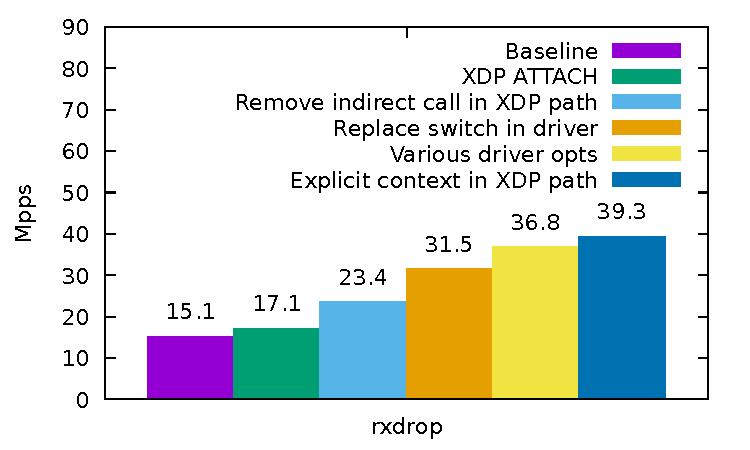
\includegraphics{results_rx.pdf}}
  \end{frame}

  \begin{frame}{Egress}
  \begin{columns}[T,onlytextwidth]
    \column{0.5\textwidth}
    \begin{itemize}
    \item Tx performance capped per HW queue $\implies$ multiple Tx
      sockets per UMEM
    \item Larger/more batching, larger descriptor rings
    \item Dedicated AF\_XDP Tx queues
    \item In-order complettion, {\tt setsockopt} {\tt XDP\_INORDER\_COMPLETION}
    \end{itemize}
    \column{0.5\textwidth}      
    \centering\resizebox{0.8\textwidth}{!}{\input{in_order.pdf_t}}
    \end{columns}
  \end{frame}

  \begin{frame}{Egress, results, data not touched}
    \resizebox{!}{\textheight}{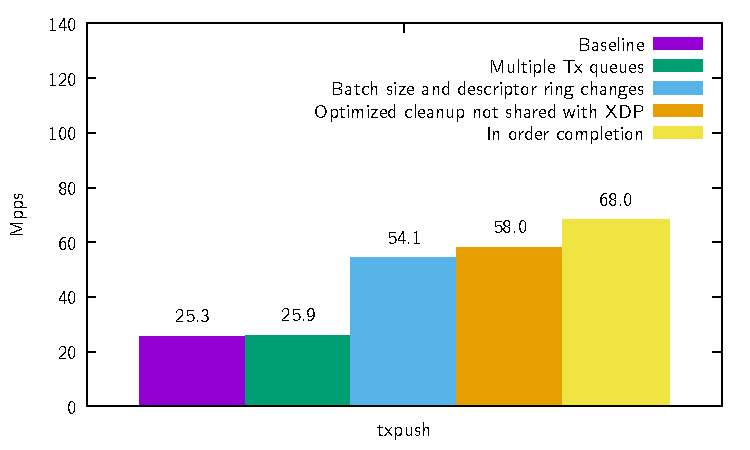
\includegraphics{results_tx.pdf}}
  \end{frame}
  \begin{frame}{Busy poll() vs run-to-completion}
    \centering\resizebox{!}{0.9\textheight}{\input{two_vs_one_core.pdf_t}}
  \end{frame}
  \begin{frame}{Busy poll() vs run-to-completion, results}
    \resizebox{!}{\textheight}{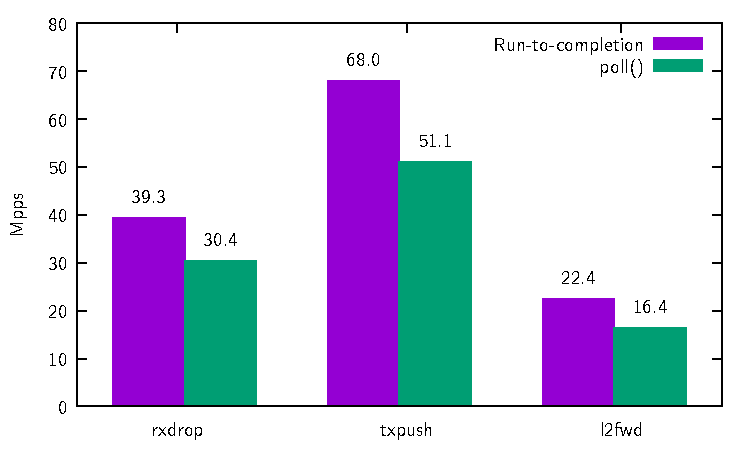
\includegraphics{results_poll.pdf}}
  \end{frame}

  \begin{frame}{Comparison with DPDK}
    \begin{itemize}
      \item Userspace, vectorized drivers
      \item ``Learning from the DPDK''
        \url{http://vger.kernel.org/netconf2018_files/StephenHemminger_netconf2018.pdf}
    \end{itemize}
  \end{frame}
  \begin{frame}{Comparison with DPDK, results}
    \resizebox{!}{\textheight}{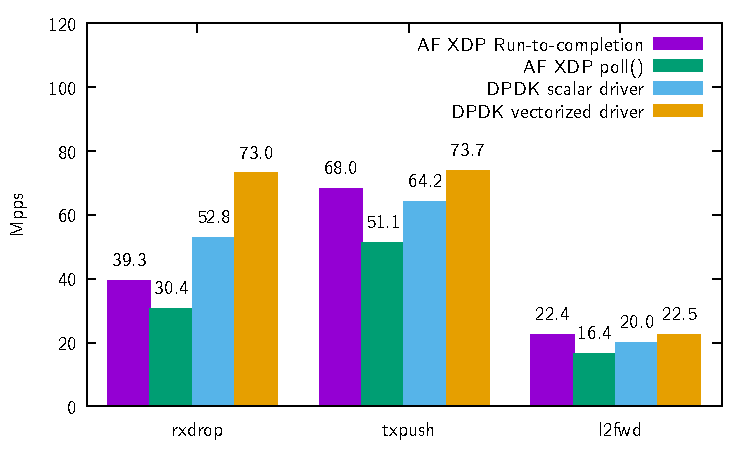
\includegraphics{results_dpdk.pdf}}
  \end{frame}

  \begin{frame}{Next steps}
    Upstream!
    \begin{itemize}
      \item XDP: switch-statement
      \item Rx/Tx: drivers
      \item Rx: {\tt XDP\_ATTTACH} and {\tt bpf\_xsk\_redirect}
      \item Tx: multiple Tx sockets per UMEM
      \item General leftovers still to-be-upstreamed: libbpf AF\_XDP
        support (easier to consume), selftest
    \end{itemize}    
  \end{frame}

  \begin{frame}{Future work}
    \begin{itemize}
    \item hugepage support, less fill ring traffic ({\tt
      get\_user\_pages})
    \item fd.io/VPP work vectors (i\$, explicit batching in function calls)
    \item ``XDP first'' drivers 
    \item collaborate/share code with RDMA (e.g. {\tt
      get\_user\_pages})
    \item Type-writer model (currently not planned)
    \end{itemize}
  \end{frame}
  % TODO Talk about built-in plus copy for tcpdump based on AF_XDP?

  \begin{frame}{Thanks!}
  \begin{columns}[T,onlytextwidth]
    \column{0.5\textwidth}
    \begin{itemize}
    \item Ilias Apalodimas
    \item Daniel Borkmann
    \item Jesper Dangaard Brouer
    \item Willem De Bruijn
    \item Eric Dumazet
    \item Alexander Duyck
    \item Mykyta Iziumtsev
    \item Jakub Kicinski
    \item Song Liu
    \end{itemize}
    
    \column{0.5\textwidth}
    \begin{itemize}
    \item David S. Miller
    \item Sridhar Samudrala
    \item Yonghong Song
    \item Alexei Starovoitov
    \item William Tu
    \item Anil Vasudevan
    \item Jingjing Wu
    \item Qi Zhang
    \end{itemize}
  \end{columns}
  \end{frame}

  \begin{frame}[standout]
    Questions?
    \resizebox{\textwidth}{!}{
\includegraphics{af_xdp_vit.pdf}}
  \end{frame}

\end{document}
